\section{Třetí týden}

\subsection{Metoda nejmenších čtverců}

\begin{multicols}{2}
    \begin{tikzpicture}
        \draw[->] (-2,0) -- (2,0) node[right] {\(x\)};
        \draw[->] (0,-2) -- (0,2) node[above] {\(y\)};
        
        \draw[blue, thick] (-1.5,-1.5) -- (1.5,1.5) node[right] {\(L = \bc{Ax \mid x \in \R^n}\)};
    
        \filldraw[red, thick] (-1, 2) circle (2pt) node[above] {$b$};
        \filldraw[red, thick] (0.5, 0.5) circle (2pt) node[right] {$P_L (b)$};
        \draw[red, dashed] (-1, 2) -- (0.5, 0.5);
    \end{tikzpicture}

\columnbreak
    Pokud $b \in L$, řešíme úlohu $Ax = b$. \\Pokud $b \not\in L$, řešíme $Ax = P_L (b)$.
    \[
        \argmin_{x \in \R^n} \| Ax - b\| = \argmin_{x \in \R^n} \| Ax - b\|^2
    \]
\end{multicols}
Důkaz.

Chceme ukázat, že $\hat x \in \underset{x \in \R^n}{\argmin} \| Ax - b^2\| \iff A^T A \hat x = A^T b$.

\enquote{$\Rightarrow$}: Ať $A \hat x = P_L (b) \stackrel{\hyperref[varNer]{(2)}}{=} b - P_{L^\perp} (b) \quad / \cdot A^T$
\[
    A^T A \hat x = A^T  b - \underbrace{A^T P_{L^\perp} (b)}_{\stackrel{?}{=0}}
\]
\[
    \rightarrow \| A^T P_{L^\perp} (b)\|^2 = \langle A^T P_{L^\perp} (b), A^T P_{L^\perp} (b)\rangle = 
    \langle \underbrace{P_{L^\perp} (b)}_{\in L^\perp}, \underbrace{(A^T)^T (A^T P_{L^\perp} (b))}_{\in L}\rangle = 0. \qed
\]

\enquote{$\Leftarrow$}: Ať $A^T A \hat x = A^T b$.\\
Ať $x \in \R^n$.
\[
    0 = \langle \underbrace{x, A^T A \hat x - A^T b}_{A^T (A \hat x - b)}\rangle = 
    \langle \underbrace{(A^T)^T x}_L, A \hat x - b\rangle \implies A \hat x - b \in L^\perp
\]
\[
    \rightarrow b = \underbrace{A \hat x}_{\in L} + \underbrace{(b-A \hat x)}_{L^\perp} 
    \stackrel{\hyperref[ortoRoz]{(c)}}{\implies} A \hat x = P_L (b). \qed
\]

\subsection{Příklad výpočtu metody nejmenších čtverců}
$
A=
\begin{bmatrix}
    1 & 0 \\
    0 & 1 \\
    1 & 1
\end{bmatrix},
b=
\begin{bmatrix}
    1 \\
    1 \\
    1 
\end{bmatrix}$.

$A^T A \hat x = A^T b$

$A^T A = 
\begin{bmatrix}
    1 & 0 & 1 \\
    0 & 1 & 1
\end{bmatrix}
\begin{bmatrix}
    1 & 0 \\
    0 & 1 \\
    1 & 1
\end{bmatrix}
=
\begin{bmatrix}
    2 & 1 \\
    1 & 2 
\end{bmatrix} 
\rightarrow \det = 3 \implies \text{existuje inverze.}$
\\

$(A^T A)^{-1} = \frac{1}{3}
\begin{bmatrix}
    2 & -1 \\
    -1 & 2 
\end{bmatrix} \implies \hat x = (A^T A)^{-1}A^T b = \frac{1}{3}
\begin{bmatrix}
    2 & -1 \\
    -1 & 2 
\end{bmatrix}
\begin{bmatrix}
    1 & 0 & 1 \\
    0 & 1 & 1
\end{bmatrix}
\begin{bmatrix}
    1 \\
    1 \\
    1 
\end{bmatrix}\\ 
= \frac{1}{3}
\begin{bmatrix}
    2 & -1 \\
    -1 & 2 
\end{bmatrix}
\begin{bmatrix}
    2 \\
    2 
\end{bmatrix} = \frac{1}{3}
\begin{bmatrix}
    2 \\
    2 
\end{bmatrix}$.

\subsection{Příklad výpočtu metody nejmenších čtverců}
V rovině jsou dány body $(0, -\frac{1}{2})^T, (1, \frac{1}{3})^T$ a $(2, \frac{2}{3})^T$. Pomocí metody nejmenších 
čtverců proložme těmito body přímku o rovnici $y = kx + q$, kde $k ,q \in \R$.

\[
\begin{rcases*}
    0k + q = -\frac{1}{2} \\
    1k + q = \frac{1}{3} \\
    2k + q = \frac{2}{3}
\end{rcases*} 
A = 
\begin{bmatrix}
    0 & 1 \\
    1 & 1 \\
    2 & 1
\end{bmatrix},
b = 
\begingroup
    \renewcommand*{\arraystretch}{1.5}
    \begin{bmatrix}
        -\frac{1}{2} \\
        \phantom{-}\frac{1}{3} \\
        \phantom{-}\frac{2}{3}
    \end{bmatrix}
\endgroup
\]

$A^T A = 
\begin{bmatrix}
    0 & 1 & 2 \\
    1 & 1 & 1
\end{bmatrix}
\begin{bmatrix}
    0 & 1 \\
    1 & 1 \\
    2 & 1 
\end{bmatrix} =
\begin{bmatrix}
    5 & 3 \\
    3 & 3
\end{bmatrix}$

$(A^T A)^{-1} = \frac{1}{6}
\begin{bmatrix}
    \phantom{-}3 & -3 \\
    -3 & \phantom{-}5
\end{bmatrix}$

\[
    \hat x = \frac{1}{6}
    \begin{bmatrix}
        \phantom{-}3 & -3 \\
        -3 & \phantom{-}5
    \end{bmatrix}
    \begin{bmatrix}
        0 & 1 & 2 \\
        1 & 1 & 1
    \end{bmatrix}
    \begingroup
        \renewcommand*{\arraystretch}{1.5}
        \begin{bmatrix}
            -\frac{1}{2} \\
            \phantom{-}\frac{1}{3} \\
            \phantom{-}\frac{2}{3}
        \end{bmatrix}
    \endgroup = \frac{1}{6}
    \begin{bmatrix}
        \phantom{-}3 & -3 \\
        -3 & \phantom{-}5
    \end{bmatrix}
    \begingroup
        \renewcommand*{\arraystretch}{1.5}
        \begin{bmatrix}
            \frac{5}{3} \\
            \frac{1}{2}
        \end{bmatrix}
    \endgroup = \frac{1}{6}
    \begingroup
        \renewcommand*{\arraystretch}{1.5}
        \begin{bmatrix}
            \phantom{-}\frac{7}{2} \\
            -\frac{5}{2}
        \end{bmatrix}
    \endgroup = \frac{1}{12}
    \begin{bmatrix}
        \phantom{-}7 \\
        -5
    \end{bmatrix}.
\]

\subsection{Věta o oddělitelnosti bodu a konvexní množiny}
\begin{multicols}{2}
    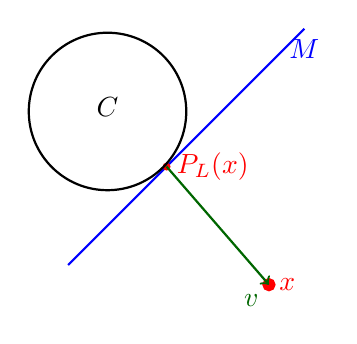
\begin{tikzpicture}  
        \draw[blue, thick] (-0.5,-0.5) -- (2.5,2.5) node[below]{$M$};

        \filldraw[red, thick] (2.05, -0.75) circle (2pt) node[right] {$x$};
        \filldraw[red, thick] (0.75, 0.75) circle (1pt) node[right] {$P_L (x)$};
        \draw[->][black!60!green, thick] (0.75, 0.75) -- (2.05, -0.75)node[below left]{$v$};
        \draw[black, thick] (0, 1.45) circle (1);
        \node at (0, 1.5) {$C$};
    \end{tikzpicture}

\columnbreak
    \hspace*{-2cm}
    $C \in \R^n$ je neprázdná uzavřená konvexní množina.
    \\
    \hspace*{-2cm}
    $x \in \R^n \setminus C \implies \text{existuje } v \in \R^n \setminus \bc{0}$ a $\alpha \in \R$ tak, že
    \\
    $\langle y, v\rangle \leq \alpha < \langle x, v\rangle, \quad \forall y \in C.$
\end{multicols}
Důkaz.\\
$v = x - P_L (x) \not=0$

\[
    \langle v, y\rangle = \langle v, P_L(x)\rangle \leq 0, \quad \forall y \in C.
\]
\[
    \langle y, v\rangle \leq \langle v, P_L (x)\rangle, \quad \forall y \in C.
\]
Položme $\alpha = \langle v, P_L (x)\rangle$.
\[
    \langle y, v\rangle \leq \alpha, \quad \forall y \in C.
\]
\[
    \langle x, v\rangle - \underbrace{\overbrace{\langle v, P_L (x)\rangle}^{\alpha}}_{\langle P_L(x), v\rangle} = 
    \langle \underbrace{x - P_L (x)}_{v}, v\rangle = \| v\|^2 > 0. \implies \alpha < \langle x, v\rangle. \qed
\]

\textbf{Důsledek:} Každá uzavřená konvexní množina v $\R^n$ je průnikem všech poloprostorů, které ji obsahují.

Důkaz sporem.

Ať neplatí: tj. existuje $C \in \R^n$ uzavřená konvexní množina tak, že není průnikem $P$ všech poloprostorů 
obsahujících $C$.

Pak $x \in P$ tak, že $x \not\in C$. Z věty o oddělitelnosti bodu a konvexní množiny existuje poloprostor $M$ takový,
že $C \subseteq M$ a $x \not= M$. Ale to je ve sporu s tím, že $x \in P. \qed$

\subsection{Příklad na použití věty o oddělitelnosti nadrovinou}
Nechť $A = 
\begin{bmatrix}
    1 & 1 \\
    2 & -1    
\end{bmatrix}$ a $b\in \R^2$. Označme
\begin{align*}
    C &= \bc{Ax \middle| x \in \R^2_+} = \bc{\alpha 
    \begin{bmatrix}
        1\\
        2    
    \end{bmatrix} + \beta
    \begin{bmatrix}
        \phantom{-}1\\
        -1
    \end{bmatrix} \mid \alpha, \beta \geq 0} \\
    K &= \bc{y \in \R^2 \mid A^T y \leq 0} \\
    &= \left\{y \in \R^2 \,\middle|\, \left\langle 
    \begin{bmatrix}
        1 \\
        2    
    \end{bmatrix}, y\right\rangle \leq 0,
    \left\langle 
    \begin{bmatrix}
        \phantom{-} 1 \\
        -1
    \end{bmatrix},y \right\rangle \leq 0\right\}.
\end{align*}

\begin{tikzpicture}[scale=2]
    \draw[->] (0,-2) -- (0,2) node[above] {\(y\)};
    \fill[green, opacity=0.3, pattern=north west lines] (0,0) -- (1,2) -- (1,-2) -- cycle;
    \fill[green, opacity=0.3, pattern=north west lines] (1,0) rectangle (2,2);
    \fill[green, opacity=0.3, pattern=north west lines] (1,0) rectangle (2,-2);

    \draw[black!40!yellow, semithick] (-0.5/4, 0.25/4) -- (-0.25/4, 0.75/4);
    \draw[black!40!yellow, semithick] (0.25/4, 0.5/4) -- (-0.25/4-0.005, 0.75/4);

    \draw[black!40!yellow, semithick] (-0.5/4, -0.25/4) -- (-0.25/4, -0.75/4);
    \draw[black!40!yellow, semithick] (0.25/4, -0.5/4) -- (-0.25/4-0.005, -0.75/4);

    \draw[black!30!blue, thick] (-2,-1) -- (2,1) node[above] {};
    \draw[black!30!blue, thick] (-2,1) -- (2,-1) node[below] {};
    \fill[blue, opacity=0.3, pattern=north east lines] (0,0) -- (-2,1) -- (-2,-1) -- cycle;
    
    \draw[->][black!40!green, thick] (0,0) -- (1,2) node[above] {};
    \draw[->][black!40!green, thick] (0,0) -- (1,-2) node[below] {};

    \draw[black!40!green, thick] (1.2,1.8) node{$C$}; 
    \draw[black!30!blue, thick] (-1.8,0.7) node{$K$}; 

    \draw[->] (-2,0) -- (2,0) node[right] {\(x\)};
    
\end{tikzpicture}

Vždy nastane jeden z případů:
\begin{enumerate}[(a)]
    \item $b \in C$
    \item $b \not\in C$
\end{enumerate}